\documentclass[11pt, twoside]{article}
\usepackage[full]{leadsheets}
\usepackage[a4paper,  hmargin=1.5cm, vmargin=3cm]{geometry}
\usepackage{multicol}
\usepackage[polish]{babel}
\usepackage{array}
\usepackage{graphicx}
\usepackage{hyperref}
\usepackage{tocloft}
\usepackage{fancyhdr}
\usepackage{tikzpagenodes}
\thispagestyle{empty}

%\usepackage[default]{lato}
%\usepackage[T1]{fontenc}

\selectlanguage{polish}
\DeclareTranslation{Polish}{leadsheets/chorus}{Ref.}
\DeclareTranslation{Polish}{leadsheets/interlude}{Przej.}
\DeclareTranslation{Polish}{leadsheets/lyrics}{tekst}
\DeclareTranslation{Polish}{leadsheets/verse}{Zwr.}
%\DeclareTranslation{Polish}{leadsheets/capo}{Kapo}
\DeclareTranslation{Polish}{leadsheets/fret}{próg}

% Tytuł spisu treści
\addto\captionspolish{\renewcommand*\contentsname{Jakieś piosenki}}

\definesongtitletemplate{custom}{%
    \let\clearpage\relax
    \ifsongmeasuring%
        {\section*}
        {\section}%
        {\songproperty{title}}%
    \begingroup\footnotesize
        \begin{tabular}{%
                @{}
                >{\raggedright\arraybackslash}p{.5\linewidth}
                @{}
                >{\raggedleft\arraybackslash}p{.5\linewidth}
                @{}
            }
            \ifsongproperty{music}{%
                Muzyka: \songproperty{music} \\%
                }{}%
            \ifsongproperty{interpret}{%
                Interpretacja: \songproperty{interpret} \\%
                }{}%
            \ifsongproperty{capo}{%
                & \capo{} \\%
                }{}%
        \end{tabular}%
        \par
    \endgroup
}

\setleadsheets{%
    title-template = custom,
    verse/numbered,
    remember-chords,
    align-chords={l},
    capo-nr-format=arabic,
    bar-shortcuts
}

\pagestyle{fancy}
\fancyhf{}
\fancyhead[L]{Jakieś piosenki}
\fancyhead[R]{\leftmark}
\fancyfoot[LE,RO]{\Large\thepage}
\fancyfoot[LO]{
\includegraphics[width=1.5cm]{kolo.png}}
\fancyfoot[RE]{
\includegraphics[width=1.5cm]{kotwica.png}}

\renewcommand{\cftdot}{\ensuremath{\sim}}
\renewcommand{\cftsecleader}{\cftdotfill{\cftdotsep}}

\begin{document}

\begin{titlepage}
    \begin{center}
        \vspace*{5cm}
        
        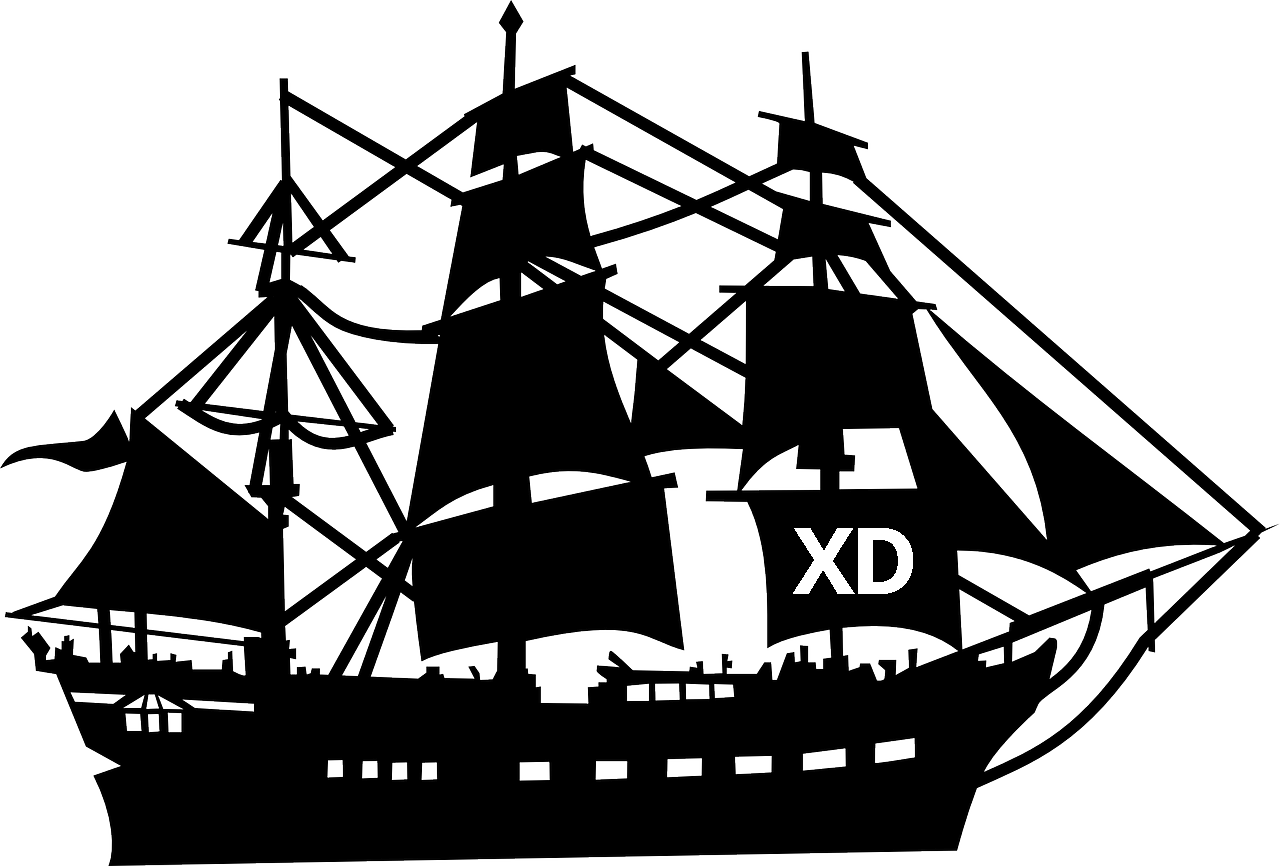
\includegraphics[height=8cm]{front-obrazek.png}

        \vspace{1.5cm}

        \Huge\textbf{Jakieś piosenki}
        
        \vspace{0.5cm}
        
        \LARGE Wydanie pierwsze
        
        \vfill

        \Large
        Wydawnictwo Kis Inkris \\
        Warszawa, 2021

        \vspace{0.5cm}

        \footnotesize
        https://github.com/dzierzanowski/spiewnik-szant

        \begin{tikzpicture}[remember picture,overlay,shift={(current page.south east)}]
            \node[anchor=south east,xshift=0cm,yshift=0cm]{
\includegraphics[width=3.5cm]{qr.png}};
        \end{tikzpicture}
    \end{center}
\end{titlepage}

\tableofcontents

\newpage
\begin{song}{title={Ballada na złe drogi}, music={EKT Gdynia}}
\begin{multicols}{2}
    \begin{intro}
        \writechord{a} \writechord{F} \writechord{d} \writechord{E} $\times 2$
    \end{intro}
    \begin{verse}
        ^{d} Na drogi złe, ^{E}dni zwyczajne \\
        ^{a} I na najwyższe ^{F} z progów \\
        ^{d} Dostaliśmy w ^{E}dłonie balladę \\
        ^{a} I pachnie jak ^{A}owoc głogu
    \end{verse}
    \begin{chorus}
        ^{d} I będzie prze^{G}biegać muzyka \\
        Czy ty ^{C}wiesz, jak to dużo po dniu ^{F} \\
        ^{d} I w wierszu nam ^{E}będzie rozkwitać \\
        Bal^{a}lada --- posag m^{A}ój \\
        ^{d} I będzie prze^{G}biegać muzyka \\
        Czy ty ^{C}wiesz, jak to dużo po dniu ^{F} \\
        ^{d} I w wierszu nam ^{E}będzie rozkwitać ballada 
    \end{chorus}
    \begin{interlude}
        \writechord{a} \writechord{F} \writechord{d} \writechord{E} $\times 2$
    \end{interlude}
    \vfill\null{}
    \columnbreak{}
    \begin{verse}
        Na ludzi o szarych obliczach \\
        Na ścieżki i wilcze doły \\
        Gdy zechcę, na głos będzie krzyczeć \\
        I w miejscu nam nie ustoi
    \end{verse}
    \begin{chorus}
        I będzie przebiegać muzyka\ldots
    \end{chorus}
    \begin{interlude}
        \writechord{a} \writechord{F} \writechord{d} \writechord{E} $\times 2$
    \end{interlude}
    \begin{verse}
        A kiedy będziemy odchodzić \\
        Hen, do Krainy Łowów \\
        Błękitne się niebo otworzy \\
        I spadnie jak owoc głogu
    \end{verse}
    \begin{chorus}
        I będzie przebiegać muzyka\ldots
    \end{chorus}
    \begin{interlude}
        \writechord{a} \writechord{F} \writechord{d} \writechord{E} $\times 2$
    \end{interlude}
\end{multicols}
\end{song}


\newpage
\begin{song}{title={Chłopcy z Botany Bay}, music={Mietek Folk}, capo=3}
\begin{multicols}{2}
    \begin{verse}
        Już nad ^{h}Hornem ^{A}zapada ^{h}noc ^{h} \\
        Wiatr na ^{h}żaglach ^{A}położył ^{D}się ^{D} \\
        |: A tam ^{G}jeszcze ^{A}korsarze na ^*{D}Bota ^{A}ny ^{h}Bay | \\
        | Upy^{G}chają ^{A}zdobycze ^{h}swe :|
    \end{verse}
    \begin{verse}
        Jolly Roger na maszcie już śpi \\
        Jutro przyjdzie z Hiszpanem się bić \\
        A korsarze znużeni na Botany Bay \\
        Za zwycięstwo dziś będa swe pić
    \end{verse}
    \begin{verse}
        Śniady Clark puchar wznosi do ust \\
        "Bracia, toast! Niech idzie na dno!" \\
        Tylko Johnny nie pije, bo kilka mil stąd \\
        Otuliło złe morze go
    \end{verse}
    \begin{verse}
        Nie podnosi kielicha do ust \\
        Zawsze on tu najgłośniej się śmiał \\
        Mistrz fechtunku z Florencji ugodził go \\
        Już nie będzie za szoty się brał
    \end{verse}
    \begin{verse}
        W starym porcie zapłacze Margot \\
        Jej kochany nie wróci już \\
        Za dezercję do panny na kei w Brisbane \\
        Oddać musiał swą głowę pod nóż
    \end{verse}
    \begin{verse}
        Tak niewielu zostało dziś ich \\
        Resztę zabrał Neptun pod dach \\
        Choć na ustach wciąż uśmiech, to w sercach lód \\
        W kuflu miesza się rum i strach
    \end{verse}
    \begin{verse}
        To ostatni chyba już rejs \\
        Cios sztyletem lub kula w pierś \\
        Bóg na szkuner w niebiosach zabierze ich \\
        Wszystkich chłopców z Botany Bay
    \end{verse}
    \begin{verse}
        Już nad Hornem zapada noc \\
        Wiatr na żaglach położył się \\
        A tam jeszcze korsarze na Botany Bay \\
        Upychają zdobycze swe
    \end{verse}
\end{multicols}
\end{song}


\newpage
\begin{song}{title={Kapitan Kidd}, music={North Cape}}
\begin{multicols}{2}
    \begin{chorus}
        Me ^{e}imię ^{h}William ^{e}Kidd \\
        Już czeka ^{a}stryk, czeka ^{D}stryk \\
        Królewski ^{e}korsarz ^{h}William ^{e}Kidd, czeka ^*{G}stry ^{D}k \\
        Me ^{G}imię ^{D}William ^{a}Kidd \\
        Zbrodni ^*{e}ogrom ^{h}nych to ^{a}mit \\
        Powró^{e}ciłem, ^{G}choć w Lon^{h}dynie ^{D/F#}czeka ^{e}stryk
    \end{chorus}
    \begin{verse}
        Mój ^{e}ojciec ^{h}uczył ^{e}mnie \\
        Jak nie ^{G}znaleźć się na ^{D}dnie \\
        Lecz los o^{e}krutny ^{D}zabrał ^{a}go ro^{h}dzinie ^{e}mej \\
        Choć biblię w ^{e}rękę ^{h}moją ^{e}kładł \\
        Morza ^{G}urok na mnie ^{D}padł \\
        I mary^{e}narzem ^{D}stałem ^{a}się, choć ^{h}czeka ^{e}stryk
    \end{verse}
    \begin{chorus}
        Me imię William Kidd\ldots
    \end{chorus}
    \begin{verse}
        Kanonier William Moore \\
        Pierwszy trafił na mój sznur \\
        Bo przeciw mnie ośmielił się on wzniecić bunt \\
        Choć dobrym strzelcem William był \\
        Pod salingiem będzie gnił \\
        Buntownik każdy skończy tak, już czeka stryk
    \end{verse}
    \begin{chorus}
        Me imię William Kidd\ldots
    \end{chorus}
    \begin{verse}
        Raz gdy było ze mną źle \\
        Obiecałem sobie, że \\
        Mądrości drogą odtąd pójdę po kres dni \\
        Lecz mój korsarski podły fach \\
        Zabił wnet o duszę strach \\
        I potępienie czeka mnie, bo czeka stryk
    \end{verse}
    \begin{chorus}
        Me imię William Kidd\ldots
    \end{chorus}
    \begin{verse}
        \textit{(wolniej)} \\
        To egzekucyjny blok \\
        Zaraz mnie ogarnie mrok \\
        Bo na mą szyję kat założy gruby sznur \\
        Więc dzisiaj ostrzec ciebie chcę \\
        Byś za przykład nie brał mnie \\
        Mądrości drogą zawsze szedł, bo czeka stryk
    \end{verse}
    \begin{chorus}
        \textit{(szybciej)} \\
        Me imię William Kidd\ldots
    \end{chorus}
\end{multicols}
\end{song}
\newpage

\newpage
\begin{song}{title={Stary bryg}, music={EKT Gdynia}}
    \begin{intro}
        \writechord{d} \writechord{a} \writechord{d} \writechord{G} $\times 2$
    \end{intro}
    \begin{verse}
        ^{d} Gdy wy^{a}pływał z ^{d}portu ^{a}stary bryg ^{d} ^{a} ^{d} ^{G} \\
        ^{d}Jego ^{C}dalszych ^{F}losów ^{C}nie znał ^{d}nikt ^{a} ^{d} ^{G} \\
        ^{d}Nikt nie wiedział ^{F}o tym, że \\
        ^{G}Statkiem-widmem ^{a}stanie się stary ^{d}bryg ^{a} ^{d} ^{G} \\
        ^{d} ^{a} ^{d} ^{G}
    \end{verse}
    \begin{chorus}
        ^{d}Hej, ^{F}ho! ^{C}na umrzyka ^{d}skrzyni \\
        ^{F}I bu^{C}telka ^{d}rumu ^{a} ^{d} ^{G} \\
        ^{d}Hej, ^{F}ho! ^{C}resztę czas u^{d}czyni \\
        ^{F}I bu^{C}telka ^{d}rumu ^{a} ^{d} ^{G} \\
        ^{d} ^{a} ^{d} ^{G}
    \end{chorus}
    \begin{verse}
        Co z załogą zrobił stary bryg \\
        Tego też nie zgadnie chyba nikt \\
        Czy zostawił w porcie ją \\
        Czy na morza dnie? Nikt nie wie gdzie
    \end{verse}
    \begin{chorus}
        Hej, ho! na umrzyka skrzyni\ldots
    \end{chorus}
    \begin{verse}
        Przepowiednia zła jest, że ho ho \\
        Kto go spotka, marny jego los \\
        Ale my nie martwmy się \\
        Hej, nie martwmy się --- rum jeszcze jest!
    \end{verse}
    \begin{chorus}
        Hej, ho! na umrzyka skrzyni\ldots $\times 2$ 
    \end{chorus}
\end{song}


\newpage
\begin{song}{title={Pójdę w połoniny (A ja wolę…)}, music={Dom o Zielonych Progach}}
    \begin{verse}
        ^{E} A ja ^{a}wolę \\
        ^{E} Na zielonej ^{a}łące ^*{G}sie ^{F}dzieć \\
        Niźli w ^{C}szarym mieście, które ^{E} głuche jest \\
        ^{F} Na moje wo^{C}łanie \\
        ^{F} Na mój niemy ^{C}krzyk \\
        ^{F} Na moją sa^{C}motność obo^{E}jętne ^{a}jest ^{G} ^{F} ^{C}
    \end{verse}
    \begin{verse}
        Pójdę w połoniny \\
        W roztańczone bujne trawy \\
        Pod rękę razem z polnym wiatrem \\
        Między szumem liści \\
        Ukryte słowa dla mnie \\
        Zanucę je głośniej, niech popłyną dalej gdzieś
    \end{verse}
    \begin{verse}
        Niech na moim niebie \\
        Rozniebieszczą się gwiazdy \\
        Niczym Mały Książę będę sobie szedł \\
        Może spotkam różę \\
        Której kolców brak \\
        Która zdradzi mi swe imię i swój uśmiech da
    \end{verse}
    \begin{interlude}
        Na na na na na\ldots
    \end{interlude}
    \begin{verse}
        Pójdę w połoniny\ldots
    \end{verse}
\end{song}


\newpage
\begin{song}{title={Premium Boy (Somebody That I Used To Know)}, music={Gotye}, interpret={808 Squad}}
\begin{multicols}{2}
    \small
    \begin{intro}
        \writechord{d} \writechord{C} \writechord{d} \writechord{C} $\times 4$
    \end{intro}
    \begin{verse}
        ^{d}Now and ^{C}then I think of ^{d}when we ^{C}were toge^{d}ther ^{C} ^{d} ^{C} \\
        ^{d} Like when you ^{C}said you felt so ^{d}happy ^{C}you could di^{d}e ^{C} ^{d} ^{C} \\
        ^{d} Told my^{C}self that you were ^{d}right for ^{C}me \\
        ^{d} But felt so ^{C}lonely in your ^{d}company ^{C} \\
        ^{d} But that was ^{C}love and it's an ^{d}ache I ^{C}still remem^{d}ber ^{C} ^{d} ^{C}
    \end{verse}
    \begin{interlude}
        \writechord{d} \writechord{C} \writechord{d} \writechord{C} $\times 4$
    \end{interlude}
    \begin{verse}
        You can get addicted to a certain kind of sadness \\
        Like resignation to the end, always the end \\
        So when we found that we could not make sense \\
        Well you said that we would still be friends \\
        But I'll admit that I was glad it was over
    \end{verse}
    \begin{chorus}
        ^{d} Bo ^{C}Michał to jest ^{B}premium ^{C}boy \\
        ^{d} Pije ^{C}kawę z mlekiem ^{B}sojowym gar^{C}dzi normal^{d}ną \\
        ^{C}Gardzi także ^*{B}herba ^{C}tą \\
        ^{d}Chyba że po^{C}słodzi cukrem ^*{B}trzcino ^{C}wym \\
        ^{d} Michał ^{C}to jest taki ^{B}premium ^{C}boy \\
        ^{d} Na jego ^{C}chlebie możesz ^{B}znaleźć tylko ^{C}  majo^{d}nez \\
        ^{C}Kiedyś zgłupiał ^{B}włączył ^{C}jazz \\
        ^{d}Potem wszedł na ^{C}łóżko i ze^{B}rzygał ^{C}się \\
        |: (bo Mi^{d}chał ^{C}--- to ^{B}premium bo^{C}y) | \\
        | ^{d}Każdy wie, że ^{C}Michał to jest ^{B}premium ^{C}boy :| \\
    \end{chorus}
    \begin{interlude}
        \writechord{d} \writechord{C} \writechord{d} \writechord{C} $\times 4$
    \end{interlude}
\end{multicols}
\end{song}



% Ostatnia strona parzysta pusta, żeby nie było tekstu na odwrocie
\clearpage{\mbox{}\pagestyle{empty}\cleardoublepage}

\end{document}
